\section{Implementación y mediciones}
\label{sec:mediciones}

\subsection{Implementación}
El filtro se monta en una placa de circuito impreso diseñada en EasyEDA. La asignación de pines del TL072CP (DIP-8) es la siguiente:
\begin{itemize}
  \item \textbf{U1 (mitad A):} pin~3 ($+$) al nodo~2; pines~1 (salida) y~2 ($-$) unidos, nodo~3.
  \item \textbf{U2 (mitad B):} pin~5 ($+$) al nodo~5; pines~7 (salida) y~6 ($-$) unidos, nodo~6.
  \item \textbf{Alimentación:} pin~8 a $+\qty{12}{\volt}$ y pin~4 a $-\qty{12}{\volt}$.
\end{itemize}
Criterios de diseño de la placa:
\begin{itemize}
  \item \textbf{Desacople:} un capacitor cerámico de \qty{100}{\nano\farad} lo más cerca posible de los pines~8 y~4, a masa, y uno electrolítico de
        \qty{10}{\micro\farad} por riel junto al conector de alimentación.
  \item \textbf{Masa:} plano de masa en la cara inferior. Las corrientes de alimentación y de desacople no deben circular por el tramo de masa de la
        entrada ni por el de la salida.
  \item \textbf{Nodos de alta impedancia} (2, 4 y 5): pistas cortas. $C_1$, $C_2$ y $R_2$ quedan junto a U2. La pista de salida no corre paralela a la
        de entrada, para no agregar un acople capacitivo que degrade la banda de rechazo, ya limitada en alta frecuencia por la fuga del Sallen--Key
        (\cref{sec:ltspice}).
  \item \textbf{Resistencias en serie:} huellas para dos resistencias por posición ($R_0$, $R_1$, $R_2$).
  \item \textbf{Conexiones y puntos de prueba:} entrada y salida en extremos opuestos de la placa (BNC o borneras con masa propia), puntos de prueba en
        los nodos 1, 3, 4 y 6, y lazos de masa para las puntas del osciloscopio.
  \item \textbf{Alimentación:} bornera de tres terminales ($+12$, GND, $-12$) con serigrafía clara. Opcionalmente, diodos en serie por riel como
        protección contra inversión de polaridad: la caída de unos \qty{0.7}{\volt} es admisible por el margen de excursión
        (\cref{sec:ao}).
  \item \textbf{Zócalo} para el TL072, de modo de poder reemplazarlo por dos TL081 o repetir mediciones con otra unidad.
\end{itemize}

\subsection{Procedimiento de medición}
\paragraph{Antes de energizar.} Se verifica la placa contra el esquema (orientación del integrado, alimentación y desacople) y la ausencia de
cortocircuitos entre rieles y masa. Se miden con multímetro las resistencias (cada par en serie como un total) y se registra el código de tolerancia de cada capacitor. La fuente
partida se ajusta a $\pm\qty{12}{\volt}$ con límite de corriente de \qty{50}{\milli\ampere} antes de conectarla; el consumo esperado es de unos
\qty{3}{\milli\ampere} por riel. Con la entrada a masa se mide la tensión continua de salida (offset).

\paragraph{Conexión.} El canal~1 del osciloscopio se conecta al borne de entrada del filtro (nodo~1) y el canal~2 a la salida (nodo~6), con puntas
$\times10$ ($\qty{10}{\mega\ohm}\parallel\approx\qty{15}{\pico\farad}$), acoplamiento DC, límite de ancho de banda de \qty{20}{\mega\hertz} y
promediado. Al tomar la referencia en el nodo~1, la magnitud medida es $V_6/V_1$: la resistencia interna del generador no interviene y el modelo de
comparación es $H_c$ con $R_s = 0$.

\paragraph{Barrido.} La medición se hizo finalmente con el modo \emph{Bode} del osciloscopio, que automatiza el barrido
(ver resultados). El plan manual, que queda como respaldo y para repetir puntos aislados, mide 34 frecuencias entre \qty{20}{\hertz} y \qty{20}{\kilo\hertz}, más densas entre \qty{700}{\hertz} y
\qty{1.5}{\kilo\hertz} (rizado, borde de paso y transición). La amplitud de entrada es de \qty{1}{\volt} eficaz hasta \qty{2}{\kilo\hertz} y de
\qty{3}{\volt} eficaces desde \qty{2.5}{\kilo\hertz}, para mejorar la relación señal/ruido donde la salida es pequeña: a esas frecuencias la
etapa~1 ya atenúa y ningún nodo se acerca a la saturación. En cada punto se miden $V_{1,\mathrm{rms}}$, $V_{6,\mathrm{rms}}$ y el retardo $\Delta t$
entre cruces por cero ascendentes. La fase es $\varphi = -360^\circ f\,\Delta t$, con $\Delta t > 0$ si la salida atrasa. Como el osciloscopio
entrega $\varphi$ módulo \ang{360} y la fase real llega a \ang{-265}, el giro se resuelve con la fase esperada; esto solo elige el número entero de
vueltas, no ajusta el dato. La planilla del repositorio incluye, para cada frecuencia, la ganancia, la salida, la fase y el $\Delta t$ esperados,
que sirven para elegir escalas y detectar errores durante la medición.

\paragraph{Ensayos adicionales.} Respuesta a una onda cuadrada de \qty{50}{\hertz} (sobrepico esperado de \qty{\vSobrepicoPy}{\percent}) y, si el
generador lo permite, ensayo de gran señal a \qty{936}{\hertz} hasta observar el recorte (esperado: $\pm\qty{10.4}{\volt}$ con $\pm\qty{12}{\volt}$,
\cref{sec:ltspice}).

\subsection{Procesamiento e incertidumbre}
Las mediciones se procesan con el notebook~04:
\begin{itemize}
  \item \textbf{Ganancia:} $G = 20\log_{10}(V_6/V_1)$. Con una precisión vertical relativa $a$ por canal (distribución rectangular),
        $u(G) \approx \frac{20}{\ln 10}\sqrt2\,a/\sqrt3$. Con $a = \qty{3}{\percent}$ resulta \qty{0.21}{\decibel}; es una cota conservadora, porque
        parte del error es común a ambos canales y se cancela en el cociente.
  \item \textbf{Fase:} $u(\varphi) = \ang{1}$. Antes de medir se corre un Bode con los dos canales en el mismo punto; lo que el instrumento mide ahí
        es su propio error entre canales, y se descuenta de todas las mediciones de la sesión.
  \item \textbf{Parámetros característicos:} se obtienen $A_{p,\max}$, $|H(\qty{1}{\kilo\hertz})|$, $|H(\qty{4}{\kilo\hertz})|$ y la frecuencia de
        \qty{-3}{\decibel} interpolando la medición. Además se ajustan $f_r$, $f_0$, $Q$ y una ganancia $K$ por mínimos cuadrados no lineales sobre
        la ganancia y la fase de los puntos con la salida a no más de \qty{30}{\decibel} por debajo de la de continua; la incertidumbre de los
        parámetros combina la covarianza del ajuste, $(J^TJ)^{-1}$ escalada por el $\chi^2$ reducido, con la variación por la elección de esa
        banda.
  \item \textbf{Capacitores:} como no se dispone de un medidor LCR, sus valores reales se estiman en forma indirecta invirtiendo la
        \cref{eq:param_circuito} con los parámetros ajustados y las resistencias medidas: $C_0 = 1/(\omega_rR_0)$,
        $C_1/C_2 = Q^2(R_1+R_2)^2/(R_1R_2)$ y $C_1C_2 = 1/(\omega_0^2R_1R_2)$. El procedimiento se validó con datos sintéticos, con desvíos
        impuestos de $+4$, $-3$ y $+\qty{6}{\percent}$ y ruido de medición realista, que se recuperaron con un error menor que
        \num{0.15} puntos porcentuales. Esos datos sintéticos no forman parte del repositorio ni de los resultados.
  \item \textbf{Retardo de grupo:} se estima de la fase medida como $-\Delta\varphi/\Delta\omega$ entre frecuencias separadas unas 0,1~década y se
        compara con el del modelo nominal y el del modelo ajustado.
\end{itemize}

\subsection{Resultados}
\IfFileExists{\resdir/valores_nb04.tex}{%
\paragraph{Condiciones.} Instrumental: osciloscopio Rigol MSO5074, generador de funciones Rigol DG1022, multímetro UNI-T UT61D+ y fuente
OWON ODP3063 (alimentación medida: $\pm\qty{\mVcc}{\volt}$). La respuesta en frecuencia se midió con el modo \emph{Bode} del osciloscopio,
con barrido logarítmico de \qty{10}{\hertz} a \qty{100}{\kilo\hertz} (\mNfrec{} frecuencias, 50 por década) y \qty{5}{\volt} pico a pico, con puntas
$\times10$ y en la misma sesión que el Nivel~III (\cref{sec:nivel3}). La calibración de canales descrita arriba mostró errores entre canales de a lo
sumo \qty{0.02}{\decibel} y \ang{0.4} hasta \qty{20}{\kilo\hertz}, que se descuentan. La respuesta al escalón se midió con una onda cuadrada de
\qty{2}{\volt} pico a pico y \qty{50}{\hertz}. Los archivos exportados por el instrumento se guardan sin modificar en
\texttt{mediciones/nivel3/}, junto con las capturas de pantalla. Las resistencias
medidas (cada par en serie como un total) son $R_0 = \qty{\mRceroMed}{\kilo\ohm}$, $R_1 = \qty{\mRunoMed}{\kilo\ohm}$ y
$R_2 = \qty{\mRdosMed}{\kilo\ohm}$, con desvíos de \qr{1}{\mDRcero}{\percent}, \qr{1}{\mDRuno}{\percent} y \qr{1}{\mDRdos}{\percent} respecto de los
valores nominales, compatibles con la tolerancia de \qty{1}{\percent} de cada resistencia más la precisión del multímetro. Con la entrada a masa,
la tensión continua de salida es de \qty{\mOffset}{\milli\volt}: la suma de las tensiones de offset de los dos seguidores, dentro de lo esperable para
el TL072 (\qty{3}{\milli\volt} típicos y \qty{10}{\milli\volt} máximos por AO).

\paragraph{Cumplimiento de la plantilla.} El filtro construido cumple la plantilla (\cref{tab:parametros_medicion,fig:mediciones_bode}). La
atenuación máxima en la banda de paso es de \qr{2}{\mApMaxMed}{\decibel}, por debajo de \qty{1}{\decibel}, y se da en el borde de \qty{1}{\kilo\hertz}.
A \qty{4}{\kilo\hertz} la atenuación es de \qr{1}{\mAcuatrokMed}{\decibel}, con más de \qty{11}{\decibel} de margen sobre los \qty{24}{\decibel}
exigidos. La frecuencia de \qty{-3}{\decibel} es de \qr{0}{\mFtresdBMed}{\hertz}, frente a \qr{0}{\mFtresdBNom}{\hertz} del diseño nominal.

\begin{table}[H]
  \centering\small
  \caption{Parámetros característicos medidos frente a la plantilla y al diseño nominal ($H_c$ con $R_s = 0$, porque se mide $V_6/V_1$).}
  \label{tab:parametros_medicion}
  \tabres{tab_parametros_medicion}
\end{table}

\begin{figure}[H]
  \centering
  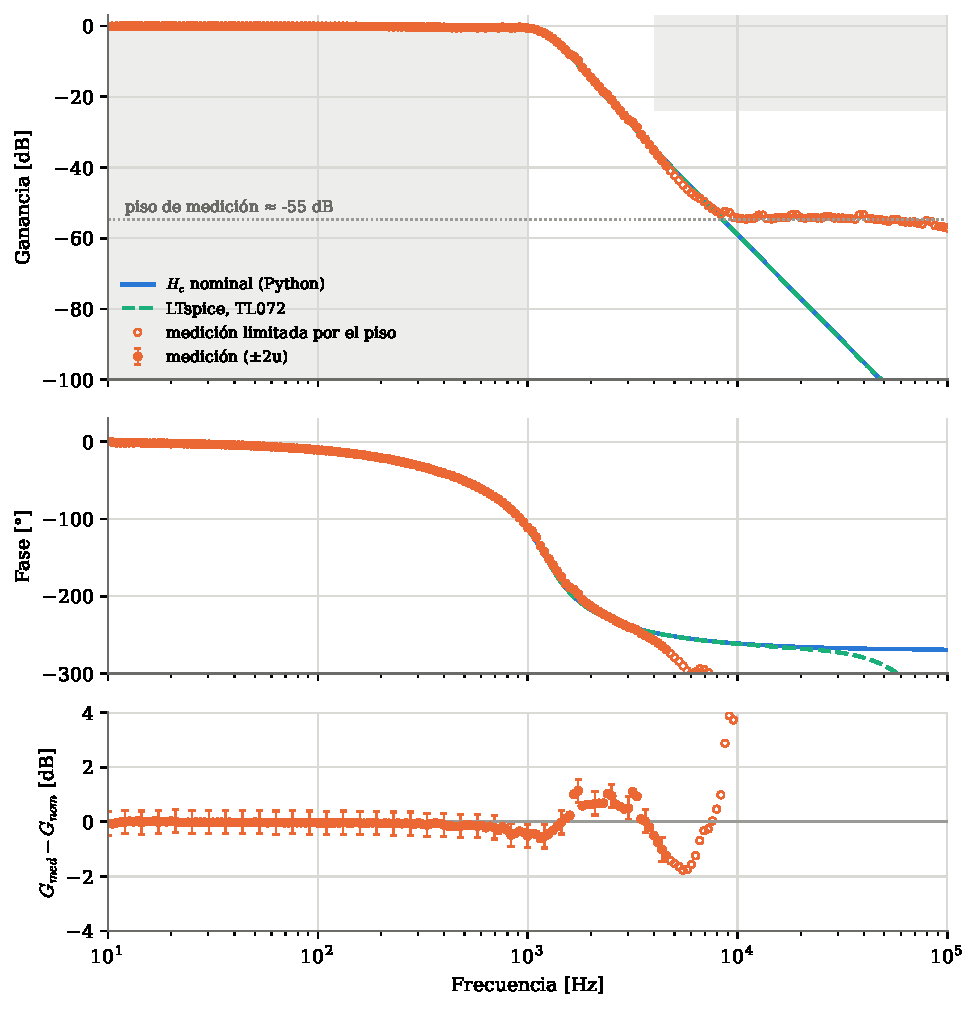
\includegraphics[width=0.95\linewidth]{fig_mediciones_bode}
  \caption{Respuesta medida (modo Bode, Rigol MSO5074) frente al modelo nominal y a LTspice con el TL072. Los puntos huecos están limitados por el
  piso de medición y no se usan en el análisis. Abajo: diferencia entre la ganancia medida y la nominal.}
  \label{fig:mediciones_bode}
\end{figure}

\paragraph{Piso de medición.} Por encima de unos \qty{9}{\kilo\hertz}, la ganancia medida se estabiliza en \qr{0}{\mPiso}{\decibel}, mientras que
el filtro debería seguir cayendo (\qty{-59}{\decibel} a \qty{10}{\kilo\hertz} y \qty{-77}{\decibel} a \qty{20}{\kilo\hertz}). Es el límite del
sistema de medición, no del filtro: con \qty{5}{\volt} pico a pico de entrada, \qty{-54}{\decibel} equivale a unos \qty{2}{\milli\volt} pico a pico,
del orden del ruido del canal visible en la captura (\qty{10}{\milli\volt\per div}). Entre \qty{4.5}{\kilo\hertz} y \qty{9}{\kilo\hertz} la
medición ya está perturbada por la suma de ese piso con la señal. Por eso solo se consideran válidos los puntos que quedan al menos
\qty{15}{\decibel} por encima del piso: \mNValidos{} puntos, hasta \qr{0}{\mFMaxValido}{\hertz}. Medir más allá requiere más amplitud de entrada,
promediado o un instrumento con más rango dinámico, y aun así la atenuación última queda limitada por la fuga del Sallen--Key (\cref{sec:ltspice}).

\paragraph{Ajuste del modelo.} Ajustando $f_r$, $f_0$, $Q$ y $K$ a la ganancia y la fase de los puntos con la salida a no más de
\qty{30}{\decibel} por debajo de la de continua (hasta \qr{0}{\mFMaxAjuste}{\hertz}) se obtiene la \cref{tab:ajuste_medicion}, con $\chi^2$ reducido
de \nr{2}{\mChiCuadRed}: el modelo describe la medición dentro de la incertidumbre supuesta, que es conservadora (\cref{fig:mediciones_paso}). La
fase es la que fija $f_r$; con la ganancia sola, $f_r$ y $Q$ están fuertemente correlacionados. La banda del ajuste agrega una incertidumbre
sistemática: cortando a \qty{-20}{\decibel} los parámetros cambian en lo que indica la \cref{tab:ajuste_medicion}, y cortando a \qty{-40}{\decibel}
entran puntos con la salida cerca del piso, cuya fase ruidosa sesga el ajuste ($f_r = \qr{0}{\mFrCorteCuarenta}{\hertz}$), por lo que no se usan.
Respecto del nominal, $f_r$ queda dentro de su incertidumbre, $f_0$ sube un \qr{1}{3.33}{\percent} y $Q$ baja un \qr{1}{7.61}{\percent}.

\begin{table}[H]
  \centering\small
  \caption{Parámetros ajustados a la ganancia y la fase medidas. La incertidumbre incluye la sistemática por la elección de la banda
  del ajuste.}
  \label{tab:ajuste_medicion}
  \tabres{tab_ajuste_medicion}
\end{table}

\begin{figure}[H]
  \centering
  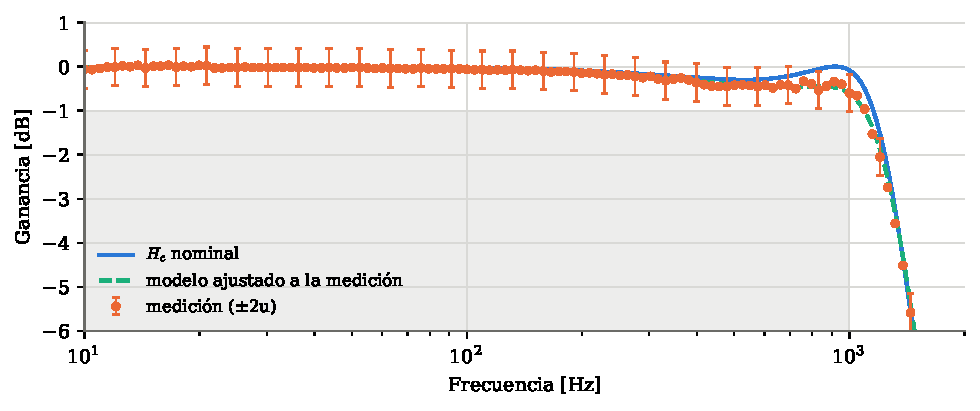
\includegraphics[width=0.92\linewidth]{fig_mediciones_paso}
  \caption{Detalle de la banda de paso: medición, modelo nominal y modelo ajustado. La zona gris es la región prohibida de la plantilla.}
  \label{fig:mediciones_paso}
\end{figure}

\paragraph{Fase.} Hasta \qty{1}{\kilo\hertz}, la fase medida difiere del modelo ajustado en \qr{2}{\mRmsResFPaso}{\degree} rms
(\cref{fig:mediciones_fase_residuo}). Por encima, con la salida cada vez más chica, el residuo crece: es de unos pocos grados hasta el límite
del ajuste (\qr{0}{\mFMaxAjuste}{\hertz}) y llega a unos \ang{20} cerca de \qty{4.5}{\kilo\hertz}, donde la salida se acerca al piso de
medición. Es el motivo por el que el ajuste se limita a la banda de \qty{-30}{\decibel}.

\begin{figure}[H]
  \centering
  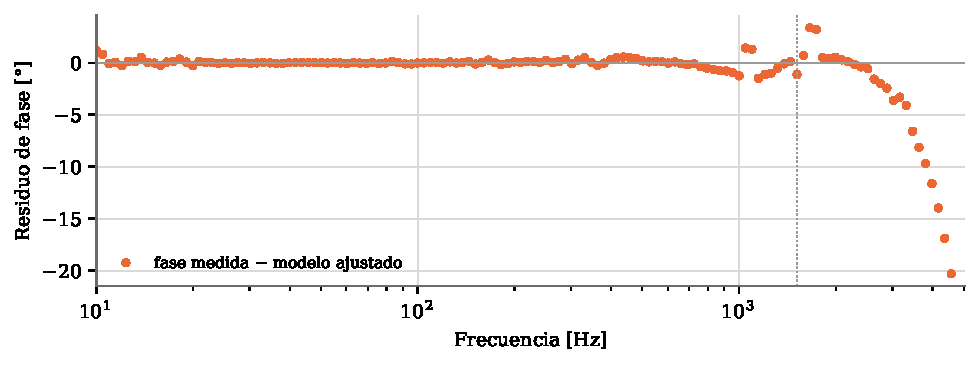
\includegraphics[width=0.9\linewidth]{fig_mediciones_fase_residuo}
  \caption{Residuo de la fase medida respecto del modelo ajustado. La línea punteada marca el paso por \ang{-180}.}
  \label{fig:mediciones_fase_residuo}
\end{figure}

\paragraph{Capacitores reales.} Invirtiendo la \cref{eq:param_circuito} con los parámetros ajustados y las resistencias medidas se estiman los
capacitores de la \cref{tab:capacitores_estimados}. Los tres capacitores llevan el código K ($\pm\qty{10}{\percent}$). $C_0$ queda prácticamente en
su valor nominal y $C_2$ \qr{1}{\mDCdos}{\percent} por encima, mientras que $C_1$ resulta \qr{1}{\mDCuno}{\percent} respecto del nominal: en el límite
de su tolerancia, con una incertidumbre de la estimación de unos \qr{0}{\mUCuno}{\percent}. Es el desvío de $C_1$ y $C_2$ en sentidos opuestos lo
que baja $Q$. Estos desvíos, junto con los de las resistencias medidas, son consistentes con el análisis de
sensibilidad: con las sensibilidades de la magnitud de la \cref{sec:sensibilidad}, predicen una variación de \qr{2}{\mDGunokPred}{\decibel} en la
ganancia a \qty{1}{\kilo\hertz}, y la medida es de \qr{2}{\mDGunokMed}{\decibel}. Como anticipaba la \cref{sec:sensibilidad}, los componentes
críticos fueron los capacitores, en este caso $C_1$ y $C_2$. Son estimaciones indirectas: heredan la incertidumbre de los parámetros ajustados,
en particular la de $f_r$, que se traslada entera a $C_0$.

\begin{table}[H]
  \centering\small
  \caption{Capacitores estimados a partir del ajuste y de las resistencias medidas. La incertidumbre combina la del ajuste y la de la medición de las
  resistencias ($\pm\qty{\mTolRMed}{\percent}$, supuesta).}
  \label{tab:capacitores_estimados}
  \tabres{tab_capacitores_estimados}
\end{table}

\paragraph{Valor del margen de diseño.} Si se aplican los mismos desvíos relativos de los componentes (capacitores estimados y resistencias medidas) a una síntesis de $H_t$ sin margen (rizado de
\qty{1}{\decibel} exacto), la atenuación máxima en la banda de paso sería de \qr{2}{\mApSinMargen}{\decibel} y el filtro \emph{no} cumpliría la
plantilla. El filtro construido, sintetizado con margen, tiene \qr{2}{\mApMaxMed}{\decibel}. La decisión de la \cref{sec:margen} se valida así con un
caso real, coherente con el Monte Carlo de esa sección: con capacitores de $\pm\qty{10}{\percent}$, como los usados (código K), el rendimiento
esperado con margen era del \qty{\vRendDiez}{\percent}, mientras que sin margen no superaba el \qty{\vRendSinMargen}{\percent} aun con capacitores de
$\pm\qty{5}{\percent}$.

\paragraph{Retardo de grupo.} Estimado a partir de la fase medida con diferencias tomadas cada 0,1~década (\cref{fig:mediciones_retardo}), el
retardo en baja frecuencia es de \qr{3}{\mTauBajaMed}{\milli\second} (nominal: \qr{3}{\mTauBajaNom}{\milli\second}) y su máximo, cerca del
borde de paso, de unos \qr{2}{\mTauMaxMed}{\milli\second} (nominal: \qr{2}{\mTauMaxNom}{\milli\second}). Por encima de
\qty{1.2}{\kilo\hertz} la estimación hereda los errores de fase del instrumento. La dispersión de los puntos en baja frecuencia es mucho menor que la
que indican las barras ($u(\varphi) = \ang{1}$ supuesta), es decir, la repetibilidad de fase del instrumento en esa zona es mejor que ese valor
conservador.

\begin{figure}[H]
  \centering
  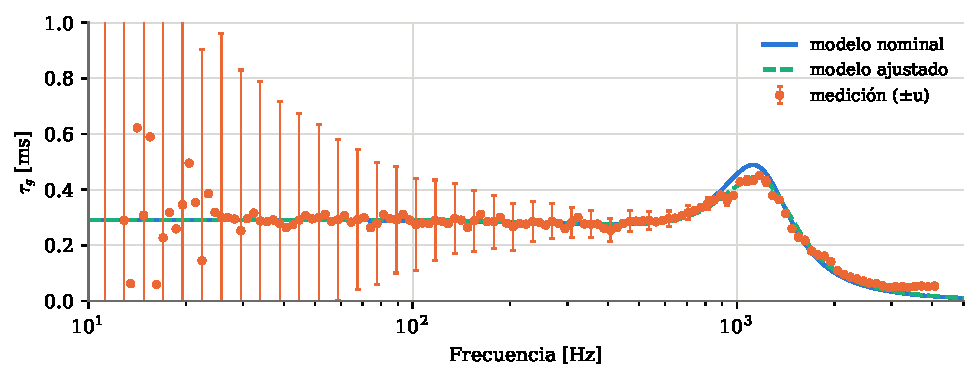
\includegraphics[width=0.9\linewidth]{fig_mediciones_retardo}
  \caption{Retardo de grupo estimado a partir de la fase medida, frente a los modelos nominal y ajustado.}
  \label{fig:mediciones_retardo}
\end{figure}

\paragraph{Respuesta al escalón.} El tiempo de subida medido, \qr{0}{\mTrMed}{\micro\second}, coincide con el del modelo ajustado con el Bode
(\qr{0}{\mTrAj}{\micro\second}) y con el nominal (\qr{0}{\mTrNom}{\micro\second}). El sobrepico medido es de
$(\nr{1}{\mSobrepicoMed} \pm \nr{1}{\mUSobrepico})\,\%$: queda entre el del modelo ajustado (\qr{1}{\mSobrepicoAj}{\percent}) y el nominal
(\qr{1}{\mSobrepicoNom}{\percent}): coincide con el primero y se aparta del segundo en menos de dos veces su incertidumbre
(\cref{fig:mediciones_escalon}). Esa incertidumbre está
dominada por la resolución vertical de la captura: \qr{1}{\mLsbmV}{\milli\volt} por nivel, el \qr{1}{2.18}{\percent} del escalón. La misma
captura incluye la salida del ecualizador del Nivel~III (\cref{sec:ec_medicion}).

\begin{figure}[H]
  \centering
  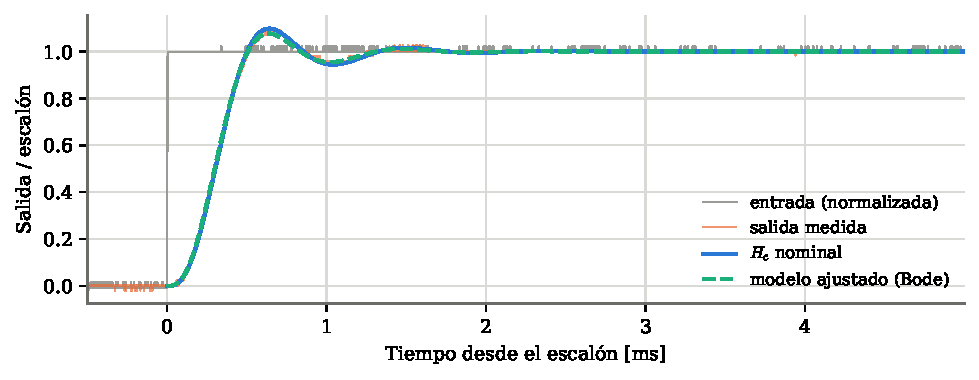
\includegraphics[width=0.9\linewidth]{fig_mediciones_escalon}
  \caption{Respuesta al escalón de \qty{2}{\volt} medida, frente a los modelos nominal y ajustado.}
  \label{fig:mediciones_escalon}
\end{figure}

\paragraph{Gran señal.} El ensayo de recorte no pudo realizarse. A \qty{936}{\hertz} la ganancia es prácticamente unitaria y, según la simulación,
la salida recorta en $\pm\qty{\vGSmaxOnce}{\volt}$; hace falta entonces una entrada de más de unos \qty{10.5}{\volt} de pico, y el generador entrega
como máximo \qty{20}{\volt} pico a pico (\qty{10}{\volt} de pico). Con esa amplitud la salida esperada es de unos \qty{10}{\volt} de pico, apenas por
debajo del recorte: el filtro no satura con ninguna señal que el generador pueda entregar, aunque el margen es chico (con $\pm\qty{\mVcc}{\volt}$ el
límite real puede quedar unas décimas de volt por debajo del simulado). El ensayo podría completarse con un amplificador previo o bajando la
alimentación, por ejemplo a $\pm\qty{9}{\volt}$, donde el recorte se espera cerca de $\pm\qty{7.5}{\volt}$.

}{%
\pendiente{cargar las mediciones en \texttt{mediciones/} y ejecutar el notebook~04.}
}
